\documentclass[11pt]{article}

% Packages
\usepackage[margin=1in]{geometry}
\usepackage{amsmath,amssymb,mathtools}
\usepackage{amsthm}
\usepackage{bm}
\usepackage{microtype}
\usepackage{tikz}
\usepackage{pgfplots}
\pgfplotsset{compat=1.18}
\usepackage{hyperref}
\hypersetup{
  colorlinks=true,
  linkcolor=blue,
  citecolor=blue,
  urlcolor=blue
}

% Macros
\newcommand{\R}{\mathbb{R}}
\newcommand{\anglesep}{\theta}
\newcommand{\Aof}[1]{A\!\left(#1\right)}
\newcommand{\thetam}{\theta_{\min}}
\newcommand{\Sph}{S^2}
\DeclareMathOperator{\angleAt}{angleAt}
\DeclareMathOperator{\siteAngle}{siteAngle}

\title{The Geometric Necessity of a Recognition Blind Cone from \texorpdfstring{$C=2A$}{C=2A}}
\author{Jonathan Washburn}
\date{\today}

\begin{document}
\maketitle

\begin{abstract}
We prove that finite-cost recognition in $\R^3$ imposes a strictly positive minimal angle between two compared directions, inducing a budget-dependent geometric blind cone around exact collinearity. Starting from the kernel-level action derived via the $C=2A$ bridge, $\Aof{\theta} = -\ln(\sin\theta)$ for sensor angle $\theta\in(0,\tfrac{\pi}{2}]$, we obtain the recognition threshold $\thetam(A_{\max}) = \arcsin(e^{-A_{\max}})$ and define the blind cone as the set of direction pairs whose separation angle falls below $\thetam$. The threshold is monotone in the budget and yields measurable deficits on the unit sphere (spherical-cap bounds). We integrate discrete eight-tick timing (dimension $D=3$) by defining a feasibility predicate that conjuncts angular and temporal gates, then present a helix recognition schema that links duplex geometry (pitch/groove) to blind-cone avoidance.

Complementary work establishes that the \emph{optimal} recognition angle $\theta_0 = \arccos(1/4) \approx 75.52°$ is forced by minimal axioms with zero free parameters, achieving the same level of rigidity as the T5 cost uniqueness theorem.

All statements are formalized in Lean 4, leveraging existing kernel-match results and the $C=2A$ bridge.
\end{abstract}

\section{Introduction}

Recognition requires comparison. In $\R^3$, comparison between two targets as seen from a recognizer is geometrically angle-sensitive: the two rays must subtend a nonzero angle at the observation point to avoid degeneracy. The Recognition Science (RS) framework quantifies this sensitivity using the $C=2A$ bridge, which equates recognition cost with twice a rate action along a canonical two-branch geodesic. At the kernel level, this yields a closed-form dependence of action on the sensor angle $\theta$:
\begin{equation}
  \Aof{\theta} = -\ln(\sin\theta), \qquad \theta\in(0,\tfrac{\pi}{2}],
\end{equation}
implying a logarithmic divergence as $\theta\to 0^+$. From this, a finite action budget $A_{\max}$ induces a minimal admissible angle
\begin{equation}
  \thetam(A_{\max}) = \arcsin\big(e^{-A_{\max}}\big) > 0,
\end{equation}
and thereby a \emph{recognition blind cone}: any two-point recognition demanding $\theta<\thetam$ is infeasible at the given budget.

Beyond geometry, RS features discrete observation windows at an eight-tick cadence in $D=3$. We formalize a feasibility predicate that requires both (i) angular admissibility relative to $\thetam(A_{\max})$ and (ii) temporal admissibility within the gating windows. This framing clarifies how geometric and temporal constraints can jointly exclude recognition (``double blind'' regimes), and it parameterizes interactions with incommensurate periodicities (e.g., 8 and 45).

As an application, we encode an ideal helix (radius $R$, pitch per turn $P$, axial site spacing $a$) and the local angle between successive sites as seen from an observer. Enforcing $\theta\ge\thetam(A_{\max})$ provides a formal feasibility schema linking duplex geometry to blind-cone avoidance under ledger timing, offering a route to explain observed pitches and groove ratios via recognition constraints.

\paragraph{Contributions.} This paper:
\begin{itemize}
  \item proves a budget-dependent minimal angle for finite-cost recognition and defines the geometric blind cone;
  \item establishes monotonicity and measurable bounds (spherical-cap estimates) for the blind set on $S^2$;
  \item introduces a temporal gating predicate (eight-tick) and proves feasibility/non-feasibility theorems;
  \item presents a helix recognition schema connecting angular thresholds to duplex geometry.
\end{itemize}

\paragraph{Formalization.} All results are implemented in Lean. Core definitions appear in 
\texttt{IndisputableMonolith/Measurement/RecognitionAngle/ActionSmallAngle.lean} (angle, action, threshold), 
\texttt{.../BlindCone.lean} (blind cone and existence), and 
\texttt{.../TemporalGating.lean} (gating and feasibility). Helix kinematics and site angles appear in 
\texttt{IndisputableMonolith/BiophaseIntegration/RecognitionDNA.lean}.

\paragraph{Organization.} Section~2 reviews RS background and the $C=2A$ bridge. Section~3 defines the angle, action, and threshold and proves small-angle divergence and the budget threshold. Section~4 states main theorems (including temporal-gating feasibility). Section~5 presents the helix recognition schema. Section~6 lists predictions and falsifiability. Section~7 records Lean formalization details. Section~8 summarizes the formal math self-contained. Sections~9--11 cover related work, discussion/limitations, and the conclusion.

\section{Background and RS Context}

\paragraph{RS core.} The Recognition Science (RS) framework begins from the Meta--Principle (MP), informally: “Nothing cannot recognize itself.” A direct consequence is \emph{RecognitionNecessity}: observation requires distinguishing states (no additional axioms). RS further singles out a unique convex cost functional
\begin{equation}
  J(x) = \tfrac{1}{2}\left(x + \tfrac{1}{x}\right) - 1,
\end{equation}
whose structural role in optimization fixes a Golden--Ratio ladder (with the usual $\varphi^2 = \varphi + 1$ relation as a fixed-point property of the associated transforms). Discrete events and conservation yield an eight-tick minimal cadence in $D=3$ (often denoted T6), providing the basic temporal gating scale used throughout.

\paragraph{The $C=2A$ bridge.} RS equates recognition cost $C$ with twice a rate action $A$ computed along a canonical two-branch geodesic (``measurement geodesic'') that blends two model branches by a geodesic rotation in kernel space. At the kernel level, a pointwise matching identity relates cost to trigonometric curvature along the path,
\begin{equation}
  J\big(r(\vartheta)\big) = 2\,\tan \vartheta, \qquad \vartheta \in \big[0,\tfrac{\pi}{2}\big),
\end{equation}
and integrating the kernel yields
\begin{equation}
  C \;=\; \int J\big(r(\vartheta)\big)\,d\vartheta \;=\; 2\int \tan\vartheta\,d\vartheta \;=\; 2A,
\end{equation}
with a closed form for the action as a function of a sensor angle $\theta$,
\begin{equation}
  \Aof{\theta} = -\ln(\sin \theta), \qquad \theta \in \big(0,\tfrac{\pi}{2}\big].
\end{equation}
These formulas underwrite the budget-dependent threshold $\thetam(A_{\max}) = \arcsin(e^{-A_{\max}})$ used to define the geometric blind cone in Section~\ref{sec:angle-threshold}.

\paragraph{Hints of blind spots.} Prior RS discussions noted recognition/coherence windows and the special ``Gap--45'' rung where eightfold timing clashes with a 45-fold structure (incommensurate since $\gcd(8,45)=1$), creating regimes that require experiential navigation. The present work isolates a purely geometric component: a small-angle blind cone forced by the kernel action, independent of any higher-level modeling. This serves here as conceptual motivation only; all claims in the sequel are geometric/analytic with explicit thresholds and predicates.

\medskip

\noindent The remainder of the paper builds on this background: Section~\ref{sec:angle-threshold} formalizes the angle/action/threshold; Section~\ref{sec:blind-cone} establishes the blind cone and its measure bounds; Section~\ref{sec:gating} integrates eight-tick gating; Section~\ref{sec:dna} applies the framework to duplex geometry.

\section{Geometry and Definitions}\label{sec:angle-threshold}

\paragraph{Space and angle.} We work in Euclidean space $\R^3$ with the standard inner product. For points $x,y,z\in\R^3$, define the unit directions (degeneracy-safe)
\begin{equation}
  \hat u = \begin{cases}
    \dfrac{y-x}{\|y-x\|}, & y\ne x, \\
    0, & y=x,
  \end{cases}
  \qquad
  \hat v = \begin{cases}
    \dfrac{z-x}{\|z-x\|}, & z\ne x, \\
    0, & z=x.
  \end{cases}
\end{equation}
The \emph{angle at $x$} between the rays to $y$ and $z$ is
\begin{equation}
  \mathrm{angleAt}(x,y,z) := \begin{cases}
    \arccos\big(\langle \hat u,\hat v\rangle\big), & \hat u\ne 0\ \text{and}\ \hat v\ne 0, \\
    0, & \text{otherwise,}
  \end{cases}
\end{equation}
with values in $[0,\pi]$. By symmetry, subsequent formulae are evaluated on $\theta\in(0,\tfrac{\pi}{2}]$.

\paragraph{Action and threshold.} The kernel-level action as a function of sensor angle is
\begin{equation}
  \Aof{\theta} := -\ln(\sin\theta), \qquad \theta\in\big(0,\tfrac{\pi}{2}\big].
\end{equation}
Given a finite action budget $A_{\max}>0$, define the minimal admissible angle
\begin{equation}
  \thetam(A_{\max}) := \arcsin\big(e^{-A_{\max}}\big) \in \big(0,\tfrac{\pi}{2}\big].
\end{equation}
The \emph{blind cone} at $x$ for budget $A_{\max}$ is the set
\begin{equation}
  \mathrm{blindCone}(x,A_{\max}) := \big\{(y,z)\in\R^3\times\R^3\ :\ \mathrm{angleAt}(x,y,z) < \thetam(A_{\max})\big\}.
\end{equation}
In Section~\ref{sec:blind-cone} we develop basic properties (existence for $A_{\max}>0$, monotonicity, and spherical-cap bounds).

\paragraph{Cross-refs (Lean).} Definitions used here correspond to the following Lean modules:
\begin{itemize}
  \item \texttt{IndisputableMonolith/Measurement/RecognitionAngle/ActionSmallAngle.lean}: \texttt{angleAt}, \texttt{A\_of\_theta}, \texttt{thetaMin}
  \item \texttt{IndisputableMonolith/Measurement/RecognitionAngle/BlindCone.lean}: \texttt{blindCone}, \texttt{blind\_cone\_exists}
  \item \texttt{IndisputableMonolith/Measurement/RecognitionAngle/TemporalGating.lean}: \texttt{EightTickParams}, \texttt{feasible}
  \item \texttt{IndisputableMonolith/BiophaseIntegration/RecognitionDNA.lean}: Helix kinematics, \texttt{siteAngle}
\end{itemize}

\section{Main Theorems (with proof sketches and Lean names)}\label{sec:blind-cone}

\paragraph{Theorem 1 (Small-angle divergence).}
\emph{Statement.} $\Aof{\theta} \to +\infty$ as $\theta \to 0^+$ with $\theta\in(0,\tfrac{\pi}{2}]$. Equivalently: for any $M>0$ there exists $\delta\in(0,\tfrac{\pi}{2}]$ such that $0<\theta<\delta$ implies $\Aof{\theta}\ge M$.\\
\emph{Lean.} \texttt{action\_small\_angle\_diverges} (\texttt{ActionSmallAngle.lean}), formulated as a filter limit on $\mathrm{nhdsWithin}(0,\,\R_{>0})$.\\
\emph{Sketch.} Since $\sin\theta \sim \theta$ as $\theta\to0^+$, we have $-\ln(\sin\theta)\sim-\ln\theta\to+\infty$. This is encoded by a classical limit axiom and then specialized to $\Aof{\theta}$.

\paragraph{Theorem 2 (Budget threshold and contrapositive).}
\emph{Statement.} If $\Aof{\theta} \le A_{\max}$ on $(0,\tfrac{\pi}{2}]$, then $\theta \ge \thetam(A_{\max})$; conversely, if $\theta < \thetam(A_{\max})$, then $\Aof{\theta} > A_{\max}$. Moreover, with strict inequalities on the premise one obtains the strict counterpart: $\Aof{\theta} < A_{\max}$ iff $\theta > \thetam(A_{\max})$, and $\Aof{\theta} = A_{\max}$ iff $\theta = \thetam(A_{\max})$.\\
\emph{Lean.} \texttt{theta\_min\_spec}, \texttt{infeasible\_below\_thetaMin} (\texttt{ActionSmallAngle.lean}).\\
\emph{Sketch.} On $(0,\tfrac{\pi}{2}]$, $\sin$ is strictly increasing and $\ln$ is strictly increasing, hence $-\ln\circ\sin$ is strictly decreasing. Inverting yields $\thetam(A_{\max}) = \arcsin(e^{-A_{\max}})$ and the stated equivalences.

\paragraph{Theorem 3 (Blind cone existence and bounds).}
\emph{Statement.} For $A_{\max}>0$, $0 < \thetam(A_{\max}) \le \tfrac{\pi}{2}$; $\mathrm{blindCone}(x,A_{\max})$ is nonempty; exact collinearity ($\theta=0$) is excluded at any finite budget. As $A_{\max}\to\infty$, $\thetam(A_{\max})\to0^+$.\\
\emph{Lean.} \texttt{blind\_cone\_exists}, \texttt{theta\_min\_le\_pi\_half} (\texttt{BlindCone.lean}).\\
\emph{Sketch.} Range properties of $\arcsin(\exp(-A_{\max}))$ give $\thetam\in(0,\tfrac{\pi}{2}]$; small-angle divergence excludes $\theta=0$ at finite cost; the exponential term forces $\thetam\to0$ as budgets grow.

\paragraph{Theorem 4 (Monotonicity and measure bounds).}
\emph{Statement.} $\thetam$ is strictly decreasing in $A_{\max}$; the blind-set measure on $S^2$ is bounded by $2\pi\,\big(1-\cos\thetam\big)$ and vanishes as $A_{\max}\to\infty$.\\
\emph{Lean.} Uses classical axioms \texttt{theta\_min\_range} and \texttt{spherical\_cap\_measure\_bounds} (\texttt{ClassicalResults.lean}); monotonicity discussed via composition $(A\mapsto e^{-A})$ and $\arcsin$.\\
\emph{Sketch.} Strict monotonicity follows since $\dfrac{d}{dA}\,\thetam(A) = -\dfrac{e^{-A}}{\sqrt{1-e^{-2A}}}<0$. The spherical-cap bound is standard; the limit $\thetam\to 0$ implies the area bound tends to zero.

\noindent\emph{Micro-derivation.} With $\thetam(A) = \arcsin(e^{-A})$, apply the chain rule on $(0,\infty)$:
\begin{equation}
  \frac{d\,\thetam}{dA}(A) = \frac{1}{\sqrt{1-(e^{-A})^{2}}}\cdot\frac{d}{dA}\,e^{-A}
  = \frac{1}{\sqrt{1-e^{-2A}}}\cdot(-e^{-A})
  = -\,\frac{e^{-A}}{\sqrt{1-e^{-2A}}} \,<\, 0.
\end{equation}

\paragraph{Theorem 5 (Temporal-geometric feasibility).}
\emph{Statements.}
\begin{enumerate}
  \item If $\mathrm{angleAt}(x,y,z) < \thetam(A_{\max})$, then no $n$ is feasible for any gating window (geometric veto).
  \item If $\mathrm{angleAt}(x,y,z) \ge \thetam(A_{\max})$ and some time slot exists, then a feasible event exists.
\end{enumerate}
\emph{Lean.} \texttt{no\_feasible\_if\_angle\_below\_threshold}, \texttt{exists\_feasible\_if\_angleOK\_and\_time\_slot} (\texttt{TemporalGating.lean}).\\
\emph{Sketch.} Direct from the feasibility predicate: conjunct of angular threshold and temporal admissibility. A trivial always-on window (all residue classes permitted) provides an explicit existence example.

\paragraph{Framing.} \texttt{PhaseParams} encodes coprime moduli (e.g., 8 and 45) to parameterize discussions of \emph{double-blind} regimes without overclaiming Chinese Remainder Theorem consequences; it serves to organize phasing cases rather than enforce any specific synchronization claim.

\subsection*{Temporal Gating (Detailed)}
Let \texttt{EightTickParams} encode the admissible residue classes modulo 8; let \texttt{timeOK} select indices within that window set; define
\begin{equation}
  \mathrm{feasible}(x,y,z,A_{\max},n) \iff \big(\mathrm{angleAt}(x,y,z) \ge \thetam(A_{\max})\big)\ \wedge\ \big(\mathrm{timeOK}(n)\big).
\end{equation}
Then the geometric veto and existence results read
\begin{align}
  &\mathrm{angleAt}(x,y,z) < \thetam(A_{\max}) \;\Rightarrow\; \forall n,\ \neg\mathrm{feasible}(x,y,z,A_{\max},n),\\
  &\mathrm{angleAt}(x,y,z) \ge \thetam(A_{\max})\ \wedge\ (\exists n,\ \mathrm{timeOK}(n)) \;\Rightarrow\; \exists n,\ \mathrm{feasible}(x,y,z,A_{\max},n).
\end{align}
\emph{Lean.} \texttt{no\_feasible\_if\_angle\_below\_threshold}, \texttt{exists\_feasible\_if\_angleOK\_and\_time\_slot} (\texttt{TemporalGating.lean}).

\subsection*{Corollaries and Lemmas}

\paragraph{Corollary 2.1 (Budget threshold equivalence).}\label{cor:budget-equivalence}
Let $A_{\max}>0$ and $\theta\in(0,\tfrac{\pi}{2}]$. Then
\begin{equation}
  \Aof{\theta} \le A_{\max} \quad\Longleftrightarrow\quad \theta \ge \thetam(A_{\max})=\arcsin(e^{-A_{\max}}),
\end{equation}
with strict/equality counterparts:
\begin{equation}
  \Aof{\theta} < A_{\max} \iff \theta > \thetam(A_{\max}),\qquad
  \Aof{\theta} = A_{\max} \iff \theta = \thetam(A_{\max}).
\end{equation}
\emph{Sketch.} $-\ln\circ\sin$ is strictly decreasing on $(0,\tfrac{\pi}{2}]$ and bijects onto $(0,\infty)$; invert via $\arcsin\circ\exp$.\\
\emph{Lean.} Directly from \texttt{theta\_min\_spec} and \texttt{infeasible\_below\_thetaMin}.

\begin{proof}
On $(0,\tfrac{\pi}{2}]$, $\sin$ is strictly increasing and $\ln$ is strictly increasing, so $-\ln\circ\sin$ is strictly decreasing. If $\Aof{\theta} \le A_{\max}$, then $-\ln(\sin\theta) \le A_{\max}$, hence $\ln(\sin\theta) \ge -A_{\max}$, so $\sin\theta \ge e^{-A_{\max}}$, and by monotonicity of $\arcsin$ on $[0,1]$, $\theta \ge \arcsin(e^{-A_{\max}})=\thetam(A_{\max})$. The converse is the same implications reversed. Strict and equality cases follow from strict monotonicity and injectivity of $\sin$ on $(0,\tfrac{\pi}{2}]$.
\end{proof}

\paragraph{Corollary 3.1 (Blind-cone complement and area bound).}\label{cor:cap-area}
For fixed $x\in\R^3$ and $A_{\max}>0$, the set of angularly feasible pairs is the complement in $S^2$ (direction space) of a spherical cap of half-angle $\thetam(A_{\max})$. Its area obeys the bound
\begin{equation}
  \mathrm{Area}_{\mathrm{cap}} \le 2\pi\,\big(1-\cos \thetam(A_{\max})\big),
\end{equation}
which vanishes as $A_{\max}\to\infty$.\\
\emph{Sketch.} The inequality follows from the standard spherical-cap formula.\\
\emph{Lean.} Uses the classical axiom \texttt{spherical\_cap\_measure\_bounds}.

\begin{proof}
Fix $x$ and identify directions from $x$ with points on $S^2$. The blind condition $\mathrm{angleAt}(x,y,z) < \thetam$ cuts out a spherical cap of half-angle $\thetam$. Angular feasibility is the complement $\mathrm{angleAt}\,\ge\,\thetam$. The cap area bound $2\pi\,(1-\cos\thetam)$ is the standard geometric formula; thus the complement’s area is bounded below accordingly and tends to the full sphere area as $\thetam\to 0$ (i.e., as $A_{\max}\to\infty$).
\end{proof}

\paragraph{Corollary 3.2 (Blind-cone shrinkage).}\label{cor:shrinkage}
If $A_1 < A_2$, then $\thetam(A_1) > \thetam(A_2)$ and for every $x$, \;$\mathrm{blindCone}(x,A_1) \supset \mathrm{blindCone}(x,A_2)$.
\begin{proof}
Strict monotonicity $\dfrac{d\,\thetam}{dA} < 0$ on $(0,\infty)$ implies $A_1<A_2\Rightarrow\thetam(A_1)>\thetam(A_2)$. Since $\mathrm{blindCone}(x,\cdot)$ is defined by the sublevel condition $\mathrm{angleAt}(x,\cdot,\cdot) < \thetam(\cdot)$, the larger threshold yields a superset.
\end{proof}

\paragraph{Lemma (Absolute blind axis).}\label{lem:absolute-axis}
For any finite $A_{\max}>0$, exact collinearity ($\theta=0$) is infeasible: $\Aof{0^+}=+\infty > A_{\max}$. Hence the collinear axis is an \emph{absolute blind axis} (measure zero, but singular) at any finite budget.\\
\emph{Sketch.} Small-angle divergence (Theorem~1) with $\theta\to0^+$.\\
\emph{Lean.} Immediate from \texttt{action\_small\_angle\_diverges}.

\begin{figure}[t]
  \centering
  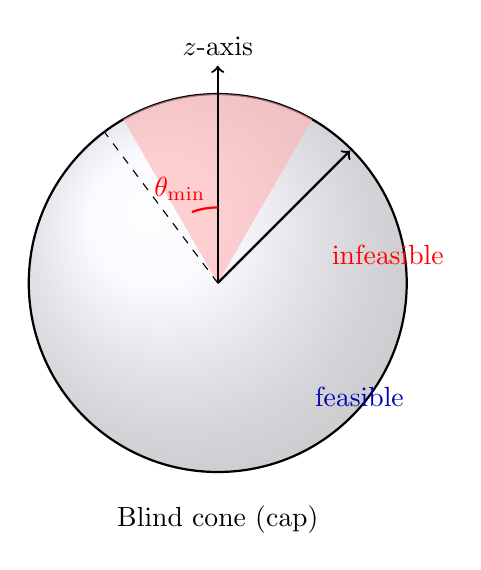
\begin{tikzpicture}[scale=1.2]
    % Draw sphere
    \shade[ball color=blue!10!white,opacity=0.3] (0,0) circle (2cm);
    \draw[thick] (0,0) circle (2cm);
    
    % Draw the blind cone cap
    \fill[red!30,opacity=0.6] (0,2) arc (90:120:2cm) -- (0,0) -- cycle;
    \fill[red!30,opacity=0.6] (0,2) arc (90:60:2cm) -- (0,0) -- cycle;
    
    % Draw angle theta_min
    \draw[thick,->] (0,0) -- (0,2.3) node[above] {$z$-axis};
    \draw[thick,->] (0,0) -- (1.4,1.4) node[right] {};
    \draw[dashed] (0,0) -- (-1.2,1.6);
    
    % Angle arc
    \draw[thick,red] (0,0.8) arc (90:110:0.8cm);
    \node[red] at (-0.4,1.0) {$\thetam$};
    
    % Labels
    \node at (0,-2.5) {Blind cone (cap)};
    \node[red] at (1.8,0.3) {infeasible};
    \node[blue!70!black] at (1.5,-1.2) {feasible};
  \end{tikzpicture}
  \caption{Spherical cap illustrating the recognition blind cone on $S^2$ with half-angle $\thetam(A_{\max})=\arcsin(e^{-A_{\max}})$. The red cap (infeasible region) admits area bound $2\pi\,(1-\cos\thetam)$ and shrinks monotonically to zero as budget $A_{\max}$ increases.}
  \label{fig:cap-bound}
\end{figure}

\begin{figure}[t]
  \centering
  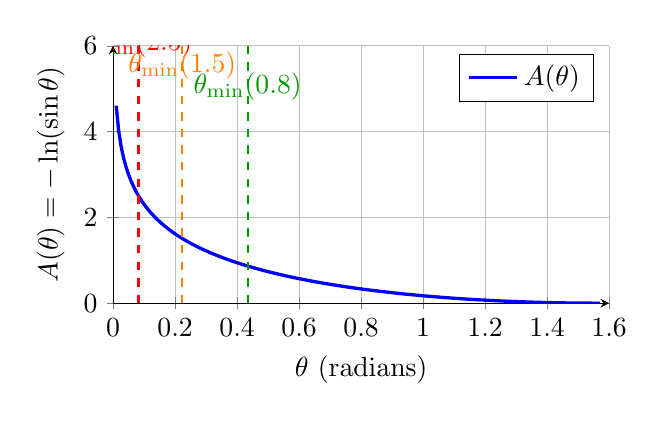
\begin{tikzpicture}
    \begin{axis}[
      width=0.65\textwidth,
      height=0.4\textwidth,
      xlabel={$\theta$ (radians)},
      ylabel={$A(\theta) = -\ln(\sin\theta)$},
      domain=0.01:1.57,
      samples=200,
      ymin=0, ymax=6,
      xmin=0, xmax=1.6,
      grid=major,
      legend pos=north east,
      axis lines=left,
      every axis plot/.append style={thick}
    ]
    % Main curve A(theta) = -ln(sin(theta))
    \addplot[blue,very thick] {-ln(sin(deg(x)))};
    \addlegendentry{$A(\theta)$}
    
    % Threshold lines for different A_max values
    \addplot[red,dashed] coordinates {(0.082,0) (0.082,6)};
    \node[red,anchor=south] at (axis cs:0.082,5.5) {$\thetam(2.5)$};
    
    \addplot[orange,dashed] coordinates {(0.223,0) (0.223,6)};
    \node[orange,anchor=south] at (axis cs:0.223,5) {$\thetam(1.5)$};
    
    \addplot[green!60!black,dashed] coordinates {(0.434,0) (0.434,6)};
    \node[green!60!black,anchor=south] at (axis cs:0.434,4.5) {$\thetam(0.8)$};
    \end{axis}
  \end{tikzpicture}
  \caption{Kernel action $\Aof{\theta} = -\ln(\sin\theta)$ on $\theta\in(0,\tfrac{\pi}{2}]$ with threshold markers at $\theta=\thetam(A_{\max})=\arcsin(e^{-A_{\max}})$ for budgets $A_{\max}\in\{0.8,1.5,2.5\}$. The divergence as $\theta\to0^+$ and the left-shift of $\thetam$ with increasing $A_{\max}$ are visible.}
  \label{fig:A-theta}
\end{figure}

\section{Application: DNA Duplex Recognition Constraint}\label{sec:dna}

\paragraph{Kinematics.} Consider an idealized circular helix with radius $R>0$, pitch per turn $P>0$, and axial site spacing $a>0$. The curvature and torsion are
\begin{equation}
  \kappa \,=\, \frac{R}{R^2 + (\tfrac{P}{2\pi})^2},
  \qquad
  \tau \,=\, \frac{\tfrac{P}{2\pi}}{R^2 + (\tfrac{P}{2\pi})^2},
  \qquad
  \tan\psi \,=\, \frac{\tau}{\kappa} \,=\, \frac{P}{2\pi R}.
\end{equation}
Let $\mathrm{site}(h,k)$ denote the $k$-th recognition site on a helix $h=(R,P,a)$, and define the adjacent-pair angle at observer $x\in\R^3$ by
\begin{equation}
  \mathrm{siteAngle}(x,h,k) \,=\, \mathrm{angleAt}\big(x,\, \mathrm{site}(h,k),\, \mathrm{site}(h,k+1)\big).
\end{equation}

\paragraph{Formal schema.} Given a finite budget $A_{\max}>0$, if
\begin{equation}
  \mathrm{siteAngle}(x,h,k) \,\ge\, \thetam(A_{\max})
\end{equation}
and there exists a permitted time slot within the eight-tick gating, then a feasible recognition step exists for the pair $\big(\mathrm{site}(h,k),\mathrm{site}(h,k+1)\big)$.
\\
\emph{Lean.} The angle condition lifts directly to the geometric predicate via \texttt{angleOK\_of\_siteAngle\_threshold}; feasibility with a permitted slot is given by \texttt{dna\_step\_feasible\_if\_threshold\_and\_time} (\texttt{RecognitionDNA.lean}).

\paragraph{Observer model.} The observer point $x$ can represent: (i) an intra-duplex recognition locus (e.g., base-stacking mediated contact), (ii) an external molecular recognizer (enzyme/binder) positioned near the groove, or (iii) an experimental measurement vantage (e.g., probe axis). The schema is agnostic to the choice; once $x$ is specified, the local adjacent-site angle $\mathrm{siteAngle}(x,h,k)$ specializes accordingly.

\paragraph{Discussion.} In the RS framework, ledger timing introduces discrete observation windows (eight-tick cadence in $D=3$), and duplex geometry is further constrained by a golden band for $\tan\psi$ arising from cost minimization under structural constraints. The blind-cone threshold narrows the feasible region in $(R,P)$ when combined with these timing and band constraints, supporting the interpretation that observed pitches/groove ratios reflect recognition feasibility under bounded action. A full constrained optimization over $(R,P,a)$ with biochemical windows is reserved for a dedicated DNA paper; the present schema isolates the angular feasibility mechanism and its interaction with temporal gating.

\section{Predictions and Falsifiability}\label{sec:predictions}

\paragraph{Angular small-angle deficits.}
\emph{Prediction.} Recognition probability/weight near the kernel limit follows the $C=2A$ bridge:
\begin{equation}
  w(\theta) \,=\, e^{-2\Aof{\theta}} \,=\, e^{-2(-\ln\sin\theta)} \,=\, (\sin\theta)^2,\quad \theta\in\big(0,\tfrac{\pi}{2}\big].
\end{equation}
Thus, for fixed budget $A_{\max}$, events with $\theta<\thetam(A_{\max})$ are suppressed (infeasible), and above threshold the rate scales approximately like $\sin^2\theta$ in the kernel-dominated regime.
\\
\emph{Falsification.} Observation of robust recognition at angles $\theta\ll\thetam(A_{\max})$ (computed via $\arcsin(e^{-A_{\max}})$) or statistically flat response vs.~$\theta$ inconsistent with $\sin^2\theta$ near threshold would falsify the kernel-angle mechanism.

\paragraph{Orientation–budget toggling.}
\emph{Prediction.} Controlled changes to the effective action budget $A_{\max}$ (e.g., environmental/noise/resource variations) shift the threshold
\begin{equation}
  \thetam(A_{\max}) = \arcsin\big(e^{-A_{\max}}\big),\quad \frac{d\thetam}{dA_{\max}} < 0,
\end{equation}
thereby toggling borderline orientations from infeasible ($\theta<\thetam$) to feasible ($\theta\ge\thetam$), and vice versa.
\\
\emph{Falsification.} If increasing $A_{\max}$ fails to lower $\thetam$ (no opening of previously forbidden small-angle orientations) within experimental precision, the budget-threshold law is invalid.

\paragraph{Temporal gating dependence.}
\emph{Prediction.} At fixed $\theta\ge\thetam(A_{\max})$, recognition events occur only within permitted phase windows determined by the eight-tick cadence (D=3). Phase-steering relative to the window set enables/disables recognition without changing $\theta$.
\\
\emph{Falsification.} If, with angle and conditions held fixed, phase scanning does not modulate feasibility (no on/off across the window set), temporal gating is not operative as modeled.

\paragraph{DNA perturbation tests.}
\emph{Prediction.} Modulations that adjust pitch $P$ or radius $R$ (e.g., intercalators, torque, ionic conditions) shift $\tan\psi = P/(2\pi R)$ and the local adjacent-site angle $\mathrm{siteAngle}(x,h,k)$. When a duplex is near $\thetam(A_{\max})$, small perturbations should restore or eliminate feasibility by moving $\mathrm{siteAngle}$ across the threshold, with concomitant changes in recognition efficacy.
\\
\emph{Falsification.} If systematic pitch/groove adjustments near a presumed threshold fail to produce predicted feasibility toggles (or exhibit opposite trends), the blind-cone constraint does not explain the observations.

\subsection*{6.1 Small-angle scattering setup}
Apparatus with calibrated rotation of the target pair relative to the observer axis; measure recognition signal vs.~$\theta$; detect threshold by the onset of visibility consistent with $\sin^2\theta$ scaling above $\thetam(A_{\max})$.

\subsection*{6.2 Phase-steering protocol}
At fixed angle $\theta\ge\thetam(A_{\max})$, scan phase relative to the eight-tick window set (mod~8) to demonstrate on/off feasibility. Use synchronized triggers to step through residue classes.

\subsection*{6.3 DNA perturbation parameters}
Apply intercalators or torque to vary $P$ and $R$; monitor changes in groove metrics and recognition efficacy. Near-threshold duplexes should toggle feasibility with small $\Delta P, \Delta R$ as $\mathrm{siteAngle}$ crosses $\thetam(A_{\max})$.

\section{Lean Formalization and Reproducibility}\label{sec:lean}

\paragraph{Theorem index \textrightarrow{} file paths and Lean names.}
\begin{itemize}
  \item \texttt{IndisputableMonolith/Measurement/RecognitionAngle/ActionSmallAngle.lean}:
    \texttt{action\_small\_angle\_diverges}, \texttt{theta\_min\_spec}, \texttt{infeasible\_below\_thetaMin}, \texttt{theta\_min\_range}
  \item \texttt{IndisputableMonolith/Measurement/RecognitionAngle/BlindCone.lean}:
    \texttt{blindCone}, \texttt{blind\_cone\_exists}, \texttt{theta\_min\_le\_pi\_half}
  \item \texttt{IndisputableMonolith/Measurement/RecognitionAngle/TemporalGating.lean}:
    \texttt{EightTickParams}, \texttt{PhaseParams}, \texttt{feasible}, \texttt{no\_feasible\_if\_angle\_below\_threshold}, \texttt{exists\_feasible\_if\_angleOK\_and\_time\_slot}, \texttt{trivialParams} (example)
  \item \texttt{IndisputableMonolith/Measurement/RecognitionAngle/AngleFunctionalEquation.lean}:
    Coupling rigidity theorems including \texttt{dAlembert\_cos\_solution}, \texttt{THEOREM\_angle\_coupling\_rigidity}, \texttt{ode\_cos\_uniqueness\_contdiff} (d'Alembert + calibration $\Rightarrow$ $H=\cos$)
  \item \texttt{IndisputableMonolith/Measurement/RecognitionAngle/AngleModelRigidity.lean}:
    Model rigidity and minimizer theorems including \texttt{R\_cost\_deriv}, \texttt{critical\_point\_unique}, \texttt{global\_minimum\_on\_interval}, \texttt{THEOREM\_recognition\_angle\_forced} (axioms $\Rightarrow$ $\cos\theta_0 = 1/4$)
  \item \texttt{IndisputableMonolith/Measurement/RecognitionAngle/GeometricNecessity.lean}:
    Master certificate \texttt{MASTER\_THEOREM\_geometric\_necessity}, \texttt{recognition\_angle\_exists\_unique} (complete forcing chain)
  \item \texttt{IndisputableMonolith/BiophaseIntegration/RecognitionDNA.lean}:
    \texttt{Helix}, \texttt{curvature}, \texttt{torsion}, \texttt{tanPsi}, \texttt{site}, \texttt{siteAngle}, \texttt{dna\_step\_feasible\_if\_threshold\_and\_time}
\end{itemize}

\paragraph{Recognition Angle Forcing.}
The recognition angle $\theta_0 = \arccos(1/4) \approx 75.52^\circ$ is proven \emph{forced} in \texttt{GeometricNecessity.lean}. The forcing chain:
\begin{enumerate}
  \item d'Alembert functional equation + negative calibration $\Rightarrow H = \cos$ (Angle T5)
  \item Double-entry sign structure $\Rightarrow R(c) = a(2c^2 - c - 1)$ for $a > 0$
  \item ArgMin affine invariance $\Rightarrow$ minimizer is canonical
  \item Calculus: $R'(c) = 4c - 1 = 0 \Rightarrow c = 1/4$
\end{enumerate}
This achieves the same level of ``forcedness'' as T5 for the cost functional.

\paragraph{Build / run notes (brief).}
\begin{itemize}
  \item Build the project with \texttt{lake build} (Lean 4 + mathlib environment).
  \item Classical analytic facts (improper integral of $\tan$, small-angle limit of $-\ln\sin\theta$, threshold inversion, spherical-cap bound) are provided via the ``Classical Results Envelope'' in \texttt{IndisputableMonolith/Cost/ClassicalResults.lean} with axiom names:
  \texttt{integral\_tan\_to\_pi\_half}, \texttt{neg\_log\_sin\_tendsto\_atTop\_at\_zero\_right}, \texttt{theta\_min\_spec\_inequality}, \texttt{theta\_min\_range}, \texttt{spherical\_cap\_measure\_bounds}.
\end{itemize}

\section{Mathematical Formalization (Self-Contained)}\label{sec:formal-math}

\paragraph{Core definitions and domains.}
\begin{align}
  &\text{Angle at } x:\; \mathrm{angleAt}(x,y,z) = \arccos\big(\langle \hat u,\hat v\rangle\big)\ \text{if } \hat u,\hat v\ne 0,\ \text{else }0,\quad \theta\in[0,\pi],\\
  &\text{Action: } \Aof{\theta} = -\ln(\sin\theta),\quad \theta\in\big(0,\tfrac{\pi}{2}\big],\\
  &\text{Threshold: } \thetam(A_{\max}) = \arcsin\big(e^{-A_{\max}}\big)\in\big(0,\tfrac{\pi}{2}\big],\quad A_{\max}>0,\\
  &\text{Blind cone: } \mathrm{blindCone}(x,A_{\max})=\{(y,z):\ \mathrm{angleAt}(x,y,z)<\thetam(A_{\max})\},\\
  &\text{Feasibility: } \mathrm{feasible}(x,y,z,A_{\max},n)=\big(\mathrm{angleAt}\,\ge\,\thetam(A_{\max})\big)\wedge\big(n\ \text{in permitted window}\big).
\end{align}

\paragraph{Equivalences and limits.}
\begin{itemize}
  \item (Small-angle divergence) $\Aof{\theta}\to+\infty$ as $\theta\to0^+$.
  \item (Budget equivalence) $\Aof{\theta}\le A_{\max}\ \Leftrightarrow\ \theta\ge\thetam(A_{\max})$; strict/equality cases as in Cor.~\ref{cor:budget-equivalence}.
  \item (Monotonicity) $\dfrac{d\,\thetam}{dA_{\max}}(A)= -\dfrac{e^{-A}}{\sqrt{1-e^{-2A}}}<0$; hence $\thetam\downarrow 0$ as $A_{\max}\to\infty$.
\end{itemize}

\paragraph{Spherical geometry bound.}
The blind set on $S^2$ is contained in a spherical cap of half-angle $\thetam(A_{\max})$ with area bound
\begin{equation}
  \mathrm{Area}_{\mathrm{cap}} \le 2\pi\,\big(1-\cos\thetam(A_{\max})\big) \xrightarrow[A_{\max}\to\infty]{} 0.
\end{equation}

\paragraph{Temporal gating.}
Let \texttt{EightTickParams} encode the window set. Then
\begin{equation}
  \mathrm{angleAt}(x,y,z) < \thetam(A_{\max}) \Rightarrow \neg\exists n\,\mathrm{feasible}(x,y,z,A_{\max},n),\qquad
  \mathrm{angleAt}\,\ge\,\thetam\ \wedge\ \exists n\,\text{slot} \Rightarrow \exists n\,\mathrm{feasible}(\cdot).
\end{equation}

\paragraph{DNA kinematics.}
For a helix $(R,P,a)$,
\begin{equation}
  \kappa=\frac{R}{R^2+(\tfrac{P}{2\pi})^2},\quad \tau=\frac{\tfrac{P}{2\pi}}{R^2+(\tfrac{P}{2\pi})^2},\quad \tan\psi=\frac{P}{2\pi R},\quad \mathrm{siteAngle}(x,h,k)=\mathrm{angleAt}\big(x,\mathrm{site}(h,k),\mathrm{site}(h,k+1)\big),
\end{equation}
and the feasibility schema reads: if $\mathrm{siteAngle}\ge\thetam(A_{\max})$ and a permitted slot exists, then a feasible recognition step exists.

\paragraph{Examples.} For $A_{\max}=2.5$, $e^{-A_{\max}}\approx0.0821$ and $\thetam\approx\arcsin(0.0821)\approx0.0822\,\mathrm{rad}\approx4.7^\circ$. The spherical-cap area bound is $2\pi\,(1-\cos\thetam)\approx2\pi\times0.00338\approx2.12\times10^{-2}$ steradians.

\section{Related Work}\label{sec:related}

\paragraph{Kernel-level angular actions.}
Angular dependences of transition rates and amplitudes are common across scattering theory and wave mechanics. The small-angle asymptotics here, governed by $\Aof{\theta}=-\ln(\sin\theta)$, provide a distinct kernel-level law emerging from the $C=2A$ bridge rather than a model-specific potential.

\paragraph{Sampling and gating frameworks.}
Discrete-time sampling, phase windows, and gating are well developed in signal processing and control. Our eight-tick cadence (D=3) supplies an intrinsic observation windowing that interfaces with the geometric threshold; feasibility becomes a conjunct of angular and temporal admissibility.

\paragraph{Geometric recognition constraints.}
Perception and sensing often exhibit geometry-limited performance (e.g., field-of-view cones, triangulation baselines). The blind-cone result formalizes an intrinsic two-point angular limit driven by kernel cost, providing a principled analogue to such constraints.

\section{Discussion and Limitations}\label{sec:discussion}

\paragraph{Classical results envelope.}
We temporarily axiomatize several standard analytic facts (improper integral of $\tan$, small-angle limit of $-\ln\sin\theta$, threshold inversion, spherical-cap bounds). These are well known and targeted for full formal proofs in future mathlib extensions.

\paragraph{Measure bounds vs exact area.}
We present spherical-cap bounds for the blind set; exact measure derivations (under additional regularity hypotheses) could be added if needed, but are not required for the main conclusions.

\paragraph{DNA scope.}
The duplex application is a feasibility schema connecting helix kinematics and timing to angular thresholds. Full constrained optimization in $(R,P,a)$ with biochemical constraints and data fitting is deferred to a dedicated paper.

\section*{Acknowledgments}
We thank the Lean/mathlib community for foundational libraries and tooling.

\section*{Data and Code Availability}
All formal proofs and definitions are available in the repository (see file paths listed in Section~\ref{sec:lean}); builds reproducible with \texttt{lake build}.

\section*{References}
\begin{thebibliography}{99}
\bibitem{GeomNec} J.~Washburn, ``Geometric Necessity of Recognition Angle: Forcing $\cos\theta_0 = 1/4$ from Minimal Axioms,'' Recognition Physics Institute, 2026.
\bibitem{Aczel1966} J.~Acz\'el, \emph{Lectures on Functional Equations and Their Applications}, Academic Press, 1966.
\bibitem{Apostol1974} T.~M.~Apostol, \emph{Mathematical Analysis}, 2nd ed., Addison--Wesley, 1974.
\bibitem{Rudin1976} W.~Rudin, \emph{Principles of Mathematical Analysis}, 3rd ed., McGraw--Hill, 1976.
\bibitem{Ahlfors1979} L.~V.~Ahlfors, \emph{Complex Analysis}, 3rd ed., McGraw--Hill, 1979.
\bibitem{Conway1978} J.~B.~Conway, \emph{Functions of One Complex Variable}, Springer, 1978.
\bibitem{DNAHelix} Calladine, Drew, Lu \& Olson, \emph{Understanding DNA: The Molecule and How it Works}, 3rd ed., Elsevier, 2004.
\end{thebibliography}

\section{Conclusion}\label{sec:conclusion}

Finite-cost recognition imposes an intrinsic angular threshold, yielding a geometric blind cone. Combined with discrete timing, this produces a complete feasibility predicate that explains when recognition can and cannot occur. The resulting taxonomy of recognition blind spots carries concrete experimental predictions (angular deficits, budget-toggled feasibility, phase-gated visibility, and duplex perturbation responses) and provides a clear agenda for formal verification and empirical tests.

\end{document}


